\section{Chandra Kirana Poetra}



 
 
\subsection{Sejarah python}

\begin{flushleft}
\qquad Python merupakan suatu bahasa pemrograman yang terinspirasi dari bahasa pemrograman ABC, bahasa pemrograman ABC inilah yang memengaruhi design dan juga pengembangan dari python. Dibuat oleh Guido Van Rossum pada tahun 1989 , python pada awalnya dikembangkan pada tahun 1980an pada saat Guido bekerja di CWI (Centrum voork Wiskunde en Informatica) sebagai programmer yang mengimplementasikan bahasa pemrograman bernama ABC, di sana dia mulai mencari bahasa seperti ABC tapi dengan akses mirip seperti AMOEBA, jadi Guido membuat sendiri bahasa pemrograman sederhana yang bisa menutup celah di ABC. Dan akhirnya pada tahun 1991, versi pertama dari python release ke publik
\end{flushleft}

\subsection{Instalasi Anaconda}
\begin{enumerate}
\item Pertama anda perlu mendownload terlebih dahulu anacondanya.
\item Visi link ini di https://www.anaconda.com/distribution/download-section
\item Setelah download anda selesai, buka file yang anda download tadi
\item Klik next
\begin{figure}[H]
\centering
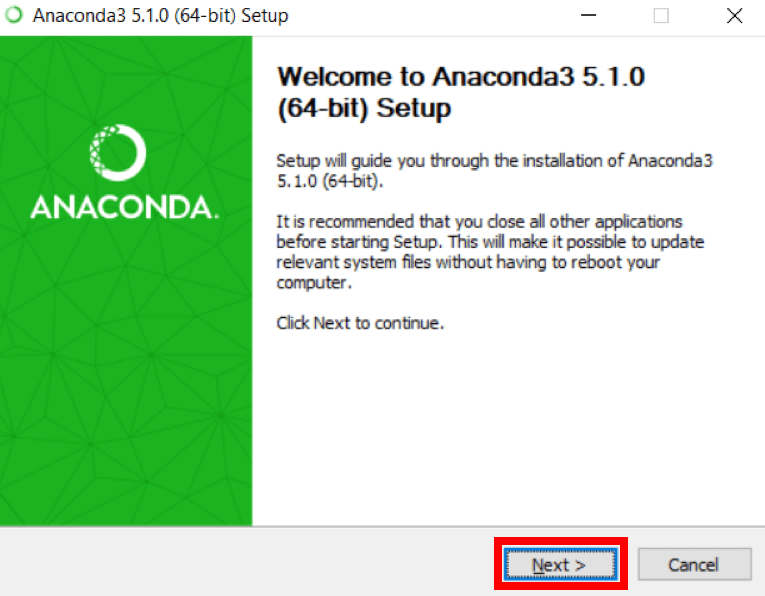
\includegraphics[width=6cm,height=6cm]{figures/1.png}
\caption{Klik Next}
\label{akhir}
\end{figure}
\item Klik I Agree
\begin{figure}[H]
\centering
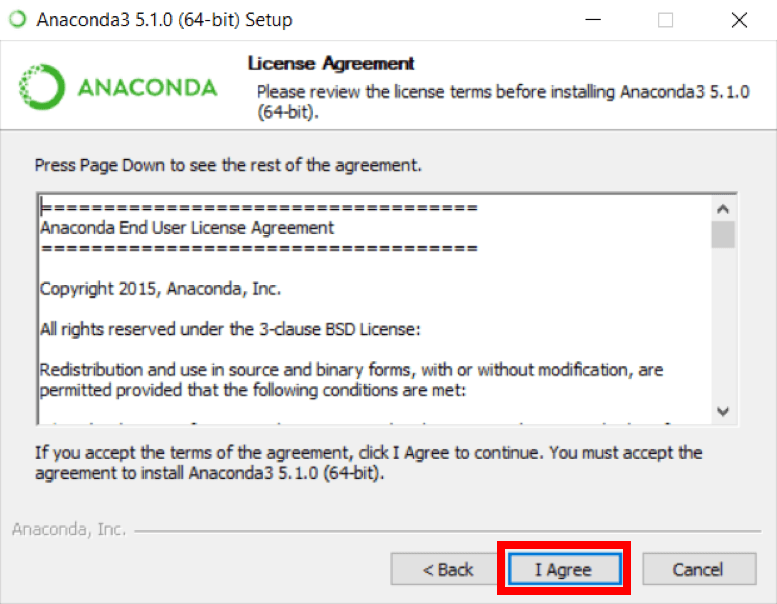
\includegraphics[width=6cm,height=6cm]{figures/2.png}
\caption{Klik I Agree}
\label{akhir}
\end{figure}
\item Pilih Just me dan klik next
\begin{figure}[H]
\centering
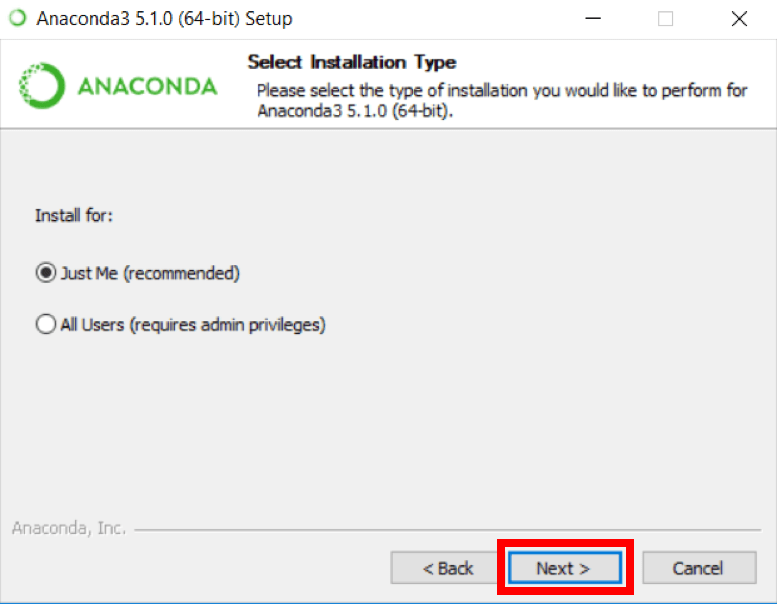
\includegraphics[width=6cm,height=6cm]{figures/3.png}
\caption{Pilih just me saja}
\label{akhir}
\end{figure}
\item Pilih directory tempat anaconda akan diinstal lalu next
\begin{figure}[H]
\centering
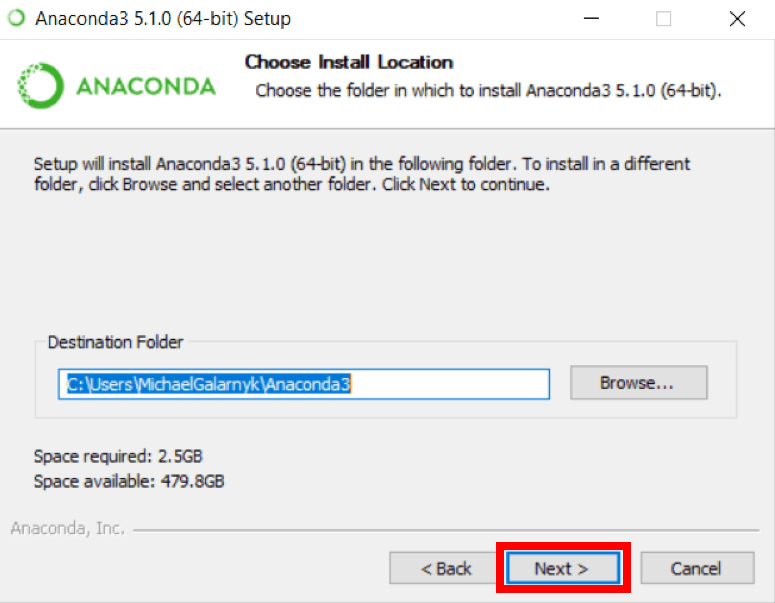
\includegraphics[width=6cm,height=6cm]{figures/4.png}
\caption{Directory tempat anaconda akan diinstalt}
\label{akhir}
\end{figure}
\item Pilih hanya opsi yang bawah saja
\begin{figure}[!htbp]
\centering
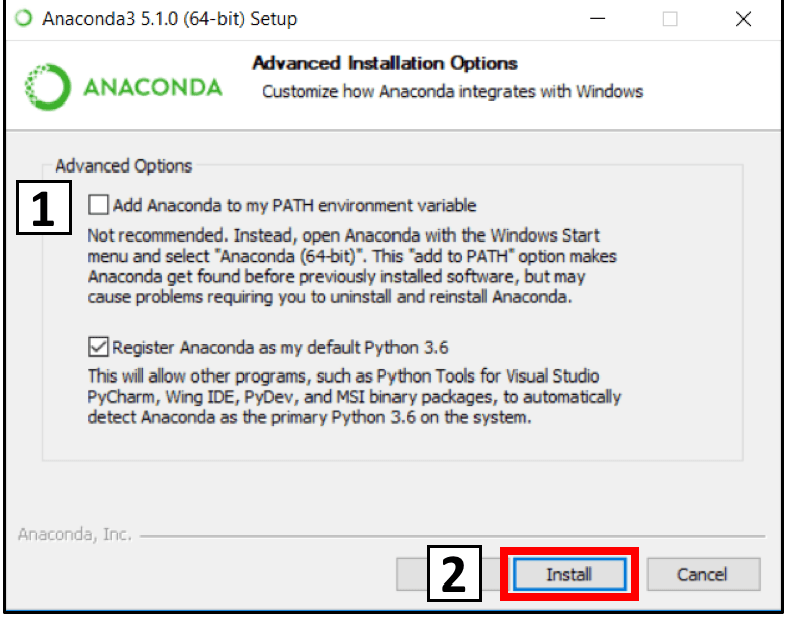
\includegraphics[width=6cm,height=6cm]{figures/5.png}
\caption{Opsi Register}
\label{akhir}
\end{figure}
\item Tunggu hingga proses selesai lalu next
\begin{figure}[H]
\centering
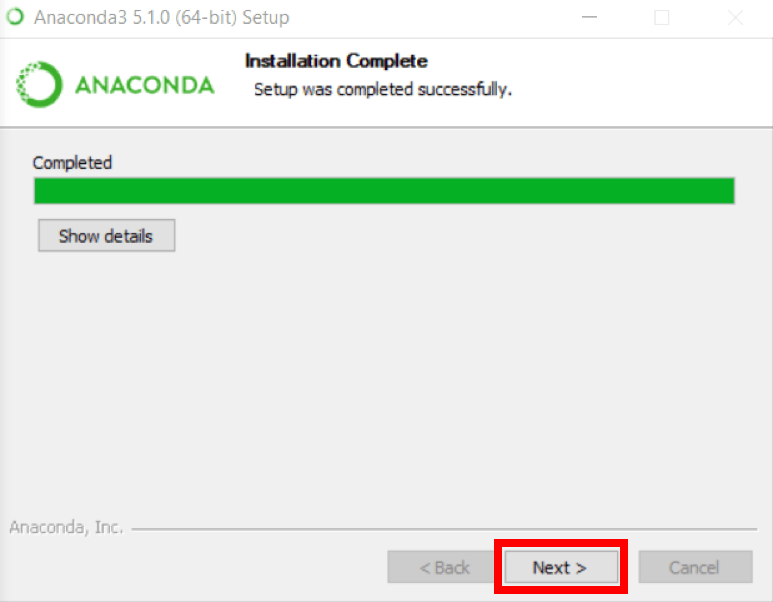
\includegraphics[width=6cm,height=6cm]{figures/6.png}
\caption{Tunggu hingga selesai}
\label{akhir}
\end{figure}
\item Opsi tambahan untuk instal visual studio code, skip saja
\begin{figure}[H]
\centering
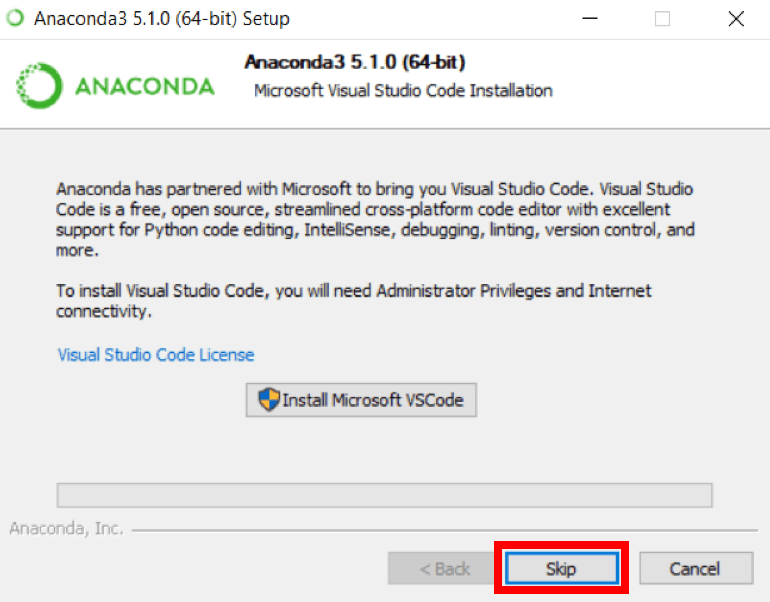
\includegraphics[width=6cm,height=6cm]{figures/7.png}
\caption{Opsi Tambahan}
\label{akhir}
\end{figure}
\item Klik saja finish
\begin{figure}[H]
\centering
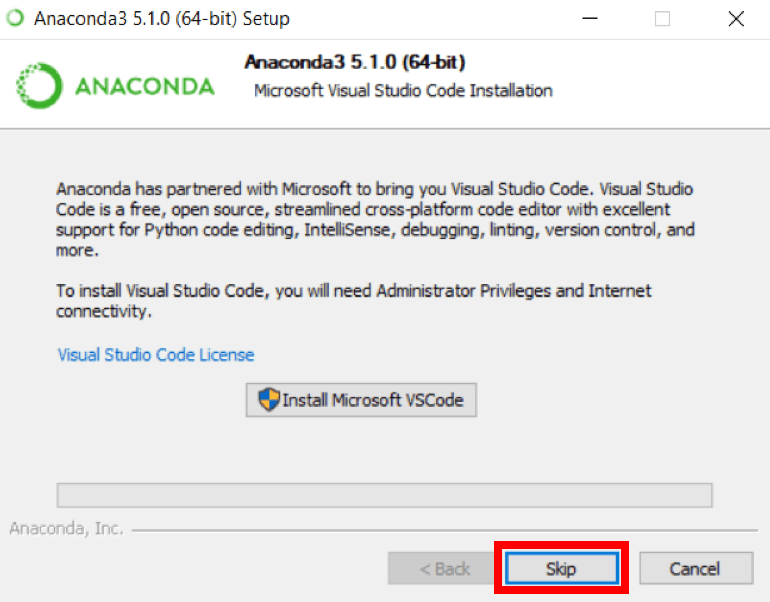
\includegraphics[width=6cm,height=6cm]{figures/7.png}
\caption{Finish}
\label{akhir}
\end{figure}
\end{enumerate}

\subsection{Spyder}
\begin{enumerate}
\item Setelah tadi install anaconda, buka aplikasinya.
\item Biasanya, spyder sudah terinstall bersamaan dengan anaconda, klik launch pada spyder
\begin{figure}[H]
\centering
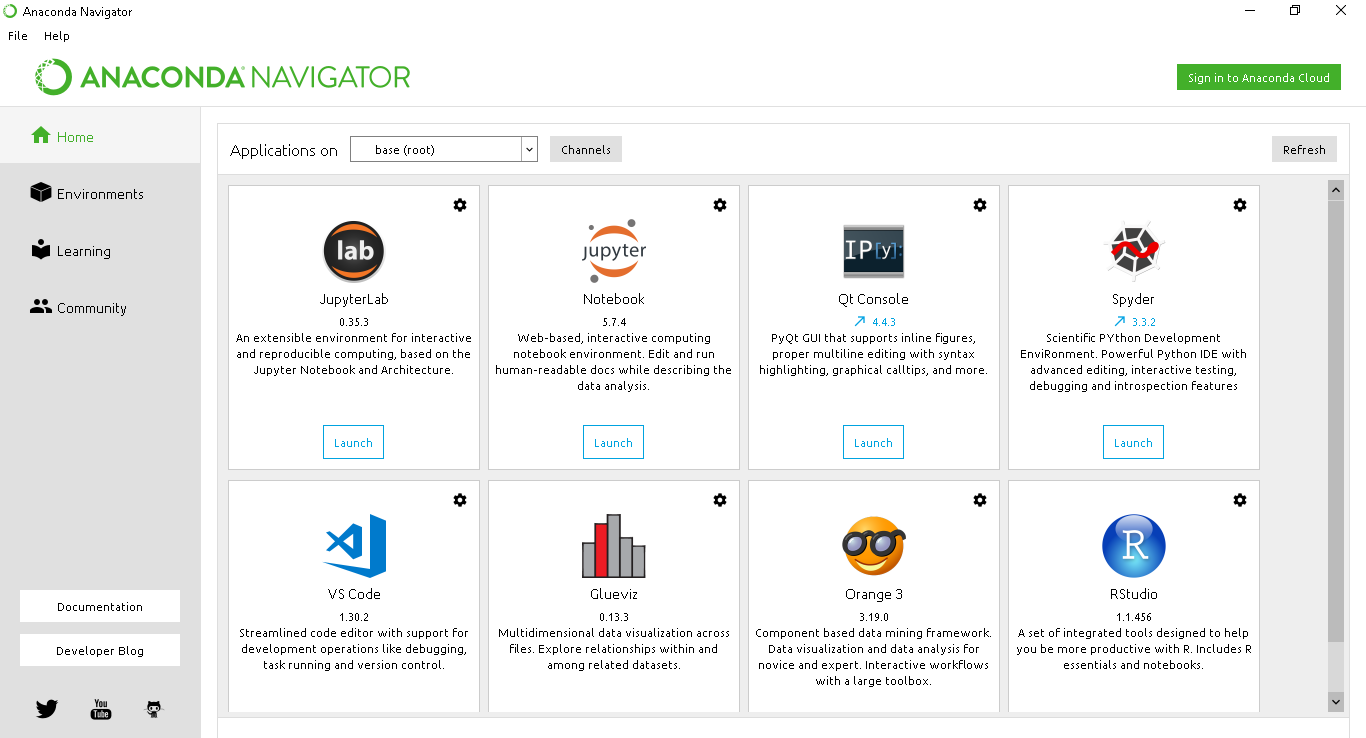
\includegraphics[width=6cm,height=6cm]{figures/9.png}
\caption{Tampilan awal anaconda}
\label{akhir}
\end{figure}
\item ketika di menu kiri, print("Hellow World") untuk percobaan pertama lalu klik simbo panah hijau untuk run, maka anda akan melihat hasilnya di console
\begin{figure}[H]
\centering
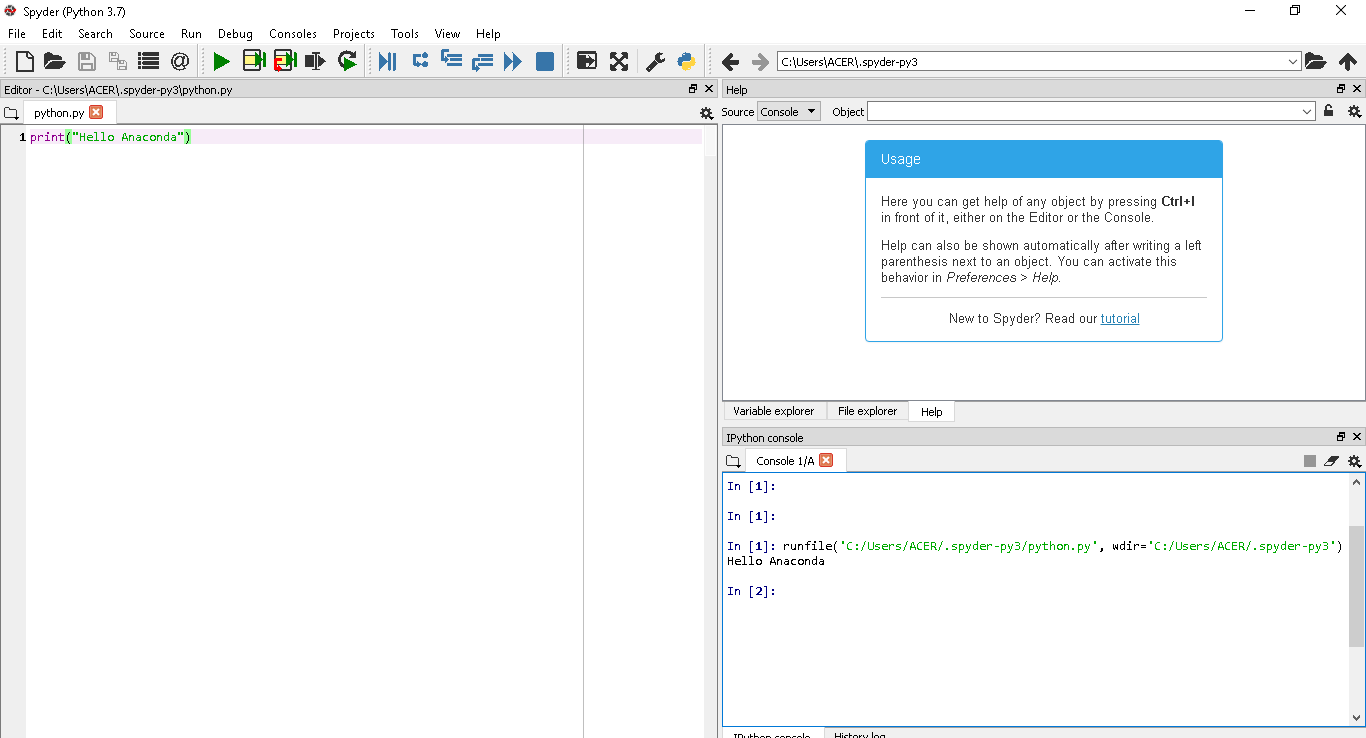
\includegraphics[width=6cm,height=6cm]{figures/10.png}
\caption{IDE Spyder}
\label{akhir}
\end{figure}

\item Output akan dihasilkan di sini
\begin{figure}[H]
\centering
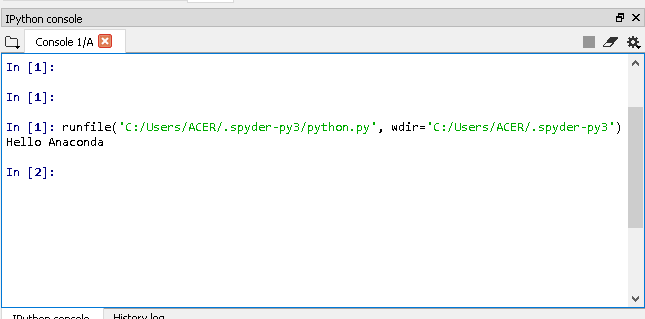
\includegraphics[width=6cm,height=6cm]{figures/11.png}
\caption{Menu Console}
\label{akhir}
\end{figure}


\end{enumerate}

%%%%%%%%%%%%%%%%%%%%%%%%%%%%%%%%%%%%%%%%%%%%%%%%%%%%%%%%%%%%%%%%%%%%%%%%%%%%%%%%%
\section{Chapter 1 | D. Irga B. Naufal Fakhri D4 TI 2C}
\subsection{Sejarah Python}
	Python adalah bahasa pemrograman interpretatif multiguna dengan filosofi perancangan yang berfokus pada tingkat keterbacaan kode. Python diklaim sebagai bahasa yang menggabungkan kapabilitas, kemampuan, dengan sintaksis kode yang sangat jelas,dan dilengkapi dengan fungsionalitas pustaka standar yang besar serta komprehensif. 

	Python diciptakan oleh Guido van Rossum di Scitchting Mathematisch Centrum (CWI) di Belanda pada tahun 1990-an. Bahasa python terinspirasi dari bahasa pemrograman ABC dan merupakan kelanjutan dari bahasa tersebut. Nama python sendiri bukan berasal dari nama ular python namun karena Guido adalah penggemar grup komedi Inggris bernama Monty Python. Guido masih menjadi penulis utama untuk python, walaupun python bersifat open source sehingga ribuan orang juga berkontribusi dalam mengembangkan python.

	Di tahun 1995, Guido melanjutkan pembuatan python di Corporation for National Research Initiative (CNRI) di Virginia Amerika, dimana dia merilis beberapa versi dari python.
Pada Mei 2000, Guido dan tim Python pindah ke BeOpen.com dan membentuk tim BeOpen PythonLabs. Di bulan Oktober pada tahun yang sama, tim python pindah ke Digital Creation (sekarang menjadi Perusahaan Zope). Pada tahun 2001, dibentuklah Organisasi Python yaitu Python Software Foundation (PSF). PSF merupakan organisasi nirlaba yang dibuat khusus untuk semua hal yang berkaitan dengan hak intelektual Python. Perusahaan Zope menjadi anggota sponsor dari PSF.

\subsection{Tanggal Rilis Python}
Semua versi python yang dirilis bersifat open source. Dalam sejarahnya, hampir semua rilis python menggunakan lisensi GFL-compatible. Berikut adalah versi major dan minor python berikut tanggal rilisnya.
\begin{itemize}
  \item Python 1.0 – Januari 1994
  \item Python 1.2 – 10 April 1995
  \item Python 1.3 – 12 Oktober 1995
  \item Python 1.4 – 25 Oktober 1996
  \item Python 1.5 – 31 Desember 1997
  \item Python 1.6 – 5 September 2000
  \item Python 2.0 – 16 Oktober 2000
  \item Python 2.1 – 17 April 2001
  \item Python 2.2 – 21 Desember 2001
  \item Python 2.3 – 29 Juli 2003
  \item Python 2.4 – 30 Nopember 2004
  \item Python 2.5 – 19 September 2006
  \item Python 2.6 – 1 Oktober 2008
  \item Python 2.7 – 3 Juli 2010
  \item Python 3.0 – 3 Desember 2008
  \item Python 3.1 – 27 Juni 2009
  \item Python 3.2 – 20 Februari 2011
  \item Python 3.3 – 29 September 2012
  \item Python 3.4 – 16 Maret 2014
  \item Python 3.5 – 13 September 2015
  \item Python 3.6 – 23 Desember 2016
\end{itemize}

\subsection{Perbedaan Python 2 dengan Python 3}
Pada Python 2 dan Python 3 memiliki kesamaan kapabilitas namun cara penggunaannya berbeda
\begin{itemize}
\item Print
\end{itemize}
Pada python2, print lebih seperti statement daripada fungsi
\begin{lstlisting}
print "Saya Belajar Python"
\end{lstlisting}
sedangkan pada python3, print digunakan sebagai fungsi
\begin{lstlisting}
print("Saya Belajar Python")
\end{lstlisting}

\begin{itemize}
\item Pembagian pada Interger
\end{itemize}
Pada Python 2, semua tipe data angka yang tidak mengandung desimal akan diperlakukan sebagai integer. Terlihat mudah pada awalnya, ketika mencoba untuk membagi kedua integer akan didapatkan tipe data float.

\begin{lstlisting}
3 / 2 = 1.5
\end{lstlisting}

Python 2 menggunakan floor division atau dibulatkan ke nilai paling rendah misalnya 1.5 jadi 1, 2.6 jadi 2 dan seterusnya. Pada Python 2.7 akan menjadi seperti ini:

\begin{lstlisting}
3
4
x = 3 / 2
print a
#Output
1
\end{lstlisting}

Untuk desimal maka tambahkan .0 setelah bilangan dan menjadi seperti ini 3.0 / 2.0  untuk mendapatkan hasil 1.5
Pada Python 3, pembagian pada bilangan integer lebih intuitif:

\begin{lstlisting}
a = 3 / 2
print(a)
#Output
1.5
\end{lstlisting}

Kita juga masih bisa melakukan 3.0 / 2.0  untuk mendapatkan 1.5 namun untuk mendapatkan floor division maka pada Python 3 gunakan //:
\begin{lstlisting}
b = 3 // 2
print(b)
#Output
1
\end{lstlisting}
Fitur pada Python 3 ini tidak bisa digunakan pada Python 2.7

\begin{itemize}
\item Dukungan Unicode
\end{itemize}

Ketika bahasa pemrograman menangani tipe data string (yang mana merupakan sekumpulan karakter), mereka bisa melakukan beberapa cara berbeda sehingga komputer dapat mengubah angka ke huruf dan simbol lain. Python 2 menggunakan alfabet ASCII secara default, sehingga ketika kita mengetik "Halo!"  maka Python 2 menangani string sebagai ASCII. Terbatas pada beberapa ratus karakter, ASCII mungkin bukan pilihan yang fleksibel untuk menangani proses encoding terutama yang non English.

Untuk menggunakan unicode yang lebih luwes, mendukung lebih dari 128,000 karakter maka kita harus mengetik u"Halo!" , dengan tambahan u  di depannya yang mana berarti Unicode.

Python 3 menggunakan Unicode secara default, yang mana menyelamatkan programmer dari tambahan kode lagi, lebih hemat waktu dan mudah untuk diisikan dan ditampilkan. Karena Unicode mendukung berbagai karakter linguistik yang beragam termasuk menampilkan emoji, penggunaan karakter secara default dengan encoding memastikan perangkat mobile didukung oleh program yang kita buat.

Jika kita ingin kode Python 3 kita mendukung Python 2, tambahkan u di depan string.

\subsection{Penggunaan Python di perusahaan dunia}
\begin{enumerate}
  \item Google adalah perusahaan besar yang menggunakan banyak kode Python di dalam mesin pencarinya. Dan mesin pencari google adalah yang paling terkenal di dunia.
  \item Youtube, situs video terbesar dan terpopuler di dunia, sebagian besar kodenya ditulis dalam bahasa Python.
  \item Facebook, media sosial terbesar di dunia, menggunakan Tornado, sebuah framework Python untuk menampilkan timeline.
  \item Instagram, siapa yang tidak kenal. Instagram menggunakan Django, framework python sebagai mesin pengolah sisi server dari aplikasinya.
  \item Pinterest, banyak menggunakan python untuk membangun aplikasinya.
  \item Dropbox, barangkali Anda adalah salah seorang pengguna layanan ini. Dropbox menggunakan python baik di sisi server maupun di sisi pengguna layanannya.
  \item Quora, salah satu situs tanya jawab terbesar di dunia, dibangun menggunakan Python.
  \item NASA, badan antariksa Amerika ini menggunakan Python untuk bidang sainsnya.
  \item NSA, badan mata – mata Amerika banyak menggunakan Python untuk analisa kriptografi dan intelijen
  \item Blender, Maya, software pembuat animasi 3D terkenal, menggunakan Python sebagai salah satu bahasa skrip pemrogramannya.
  \item Raspberry Pi, komputer mini yang banyak digunakan sebagai mikrokontroller, menggunakan Python sebagai bahasa utamanya.
  \item ESRI, produsen terkenal pembuat software pemetaan GIS banyak menggunakan Python di produknya.
\end{enumerate}
Untuk lebih lengkapnya bisa mengunjungi www.python.org/about/success/



\subsection{Cara menginstall Anaconda}
\begin{enumerate}
  \item Pastikan anda telah menginstall python dan anda mengetahui versi dari python yang telah anda install
  \item Download Anaconda dari website www.anaconda.com/distribution
  \item pilih sesuai dengan versi python anda, jika versi anda python3 maka pilih python3
  \item Setelah itu buka file yang telah anda download
  \item Setelah muncul gambar dibawah ini, tekan next
\begin{figure}[!htbp]
  \centering
  \includegraphics[height=3cm]{chapters/gambar/install1.jpg}
  \caption{Tampilan Instalasi 1}
\end{figure}

  \item Baca license agreement lalu tekan 'I Agree'
\begin{figure}[!htbp]
  \centering
  \includegraphics[height=3cm]{chapters/gambar/install2.jpg}
  \caption{Tampilan Instalasi 2}
\end{figure}

  \item Setelah itu pilih mau diinstall pada user yang sedang anda pakai atau kesemua user, direkomendasikan untuk memilih just me yaitu hanya user yang sedang dipakai saja
\begin{figure}[!htbp]
  \centering
  \includegraphics[height=3cm]{chapters/gambar/install3.jpg}
  \caption{Tampilan Instalasi 3}
\end{figure}

  \item Catat tempat dimana anda akan menginstall anaconda, lalu tekan 'Next'
\begin{figure}[!htbp]
  \centering
  \includegraphics[height=3cm]{chapters/gambar/install4.jpg}
  \caption{Tampilan Instalasi 4}
\end{figure}

  \item Setelah itu anda diberi pilihan, direkomendasikan untuk tidak mengubah pilihan tersebut, lalu tekan 'Install'
\begin{figure}[!htbp]
  \centering
  \includegraphics[height=3cm]{chapters/gambar/install5.jpg}
  \caption{Tampilan Instalasi 5}
\end{figure}

  \item Tunggu sampai instalasi selesai
\begin{figure}[!htbp]
  \centering
  \includegraphics[height=3cm]{chapters/gambar/install6.jpg}
  \caption{Tampilan Instalasi 6}
\end{figure}

  \item Setelah selesai tekan 'Next'
\begin{figure}[!htbp]
  \centering
  \includegraphics[height=3cm]{chapters/gambar/install7.jpg}
  \caption{Tampilan Instalasi 7}
\end{figure}

  \item Setelah itu ada opsi untuk memilih untuk meinstall visual studio code, jika anda berminat klik 'Install VSCode' jika tidak tekan 'Skip'
\begin{figure}[!htbp]
  \centering
  \includegraphics[height=3cm]{chapters/gambar/install8.jpg}
  \caption{Tampilan Instalasi 8}
\end{figure}

  \item Tekan 'Finish' untuk menyelesaikan instalasi
\begin{figure}[!htbp]
  \centering
  \includegraphics[height=3cm]{chapters/gambar/install9.jpg}
  \caption{Tampilan Instalasi 9}
\end{figure}

\end{enumerate}

\subsection{Cara menggunakan Spyder pada Anaconda}
Pertama buka aplikasi Anaconda sampai muncul seperti ini
\begin{figure}[!htbp]
  \centering
  \includegraphics[height=3cm]{chapters/gambar/gambaranaconda.jpg}
  \caption{Tampilan awal Anaconda}
\end{figure}

Setelah itu tekan Launch dibawah logo Spyder
Tunggu sampai muncul seperti ini
\begin{figure}[!htbp]
  \centering
  \includegraphics[height=3cm]{chapters/gambar/gambarspider.jpg}
  \caption{Tampilan spider}
\end{figure}

\subsection{Membuat Hello World di Spyder}
Setelah membuka spyder seperti gambar di section sebelumnya tekan menu File lalu klik New File atau bisa menggunakan kombinasi tombol Ctrl + N sampai muncul seperti ini

\begin{figure}[!htbp]
  \centering
  \includegraphics[height=3cm]{chapters/gambar/gambarnewfile.jpg}
  \caption{Tampilan new file pada spider}
\end{figure}

Karena kita menggunakan Python3.7 maka kita menggunakan funsi print() untuk memunculkan teks Hello World yang akan kita buat, tuliskan print("Hello World") pada teks editor di Spyder

\begin{figure}[!htbp]
  \centering
  \includegraphics[height=3cm]{chapters/gambar/gambarprint.jpg}
  \caption{print("Hello World")}
\end{figure}

setelah itu tekan tombol play berwarna hijau diatas, karena kita belum save file yang kita buat maka akan muncul dialog simpan file, pilih tempat dan nama file yang akan disimpan contohnya helloworld.py

\begin{figure}[!htbp]
  \centering
  \includegraphics[height=3cm]{chapters/gambar/helloworld.jpg}
  \caption{Dialog simpan file}
\end{figure}

setelah itu tekan run maka hasil dari program yang kita buat tadi ada dibagian console yang berada di pinggir kanan bawah

\begin{figure}[!htbp]
  \centering
  \includegraphics[height=3cm]{chapters/gambar/hasil.jpg}
  \caption{Hasil Program}
\end{figure}


%%%%%%%%%%%%%%%%%%%%%%%%%%%%%%%%%%%%%%%%%%%%%%%%%%%%%%%%%%%%%%%%%%%%%%%%%%%%%%%%%%%
\section{Bakti Qilan Mufid}
\subsection{Resume Sejarah Python}
\begin{flushleft}
\qquad Bahasa pemrograman Python dirilis pertama kali oleh Guido van Rossum di tahun 1991, yang sudah dikembangkan sejak tahun 1989. Awal pemilihan nama Python tidak secara langsung berasal dari nama ular piton, tapi sebuah acara humor di BBC pada era 1980an dengan judul “Monty Python’s Flying Circus“. Monty Python adalah kelompok lawak yang membawakan acara tersebut. Kebetulan Guido van Rossum adalah penggemar dari acara ini. Pada tahun 1994, Python 1.0 dirilis, yang diikuti dengan Python 2.0 pada tahun 2000. Python 3.0 keluar pada tahun 2008.
\end{flushleft}
\subsection{Perbedaan Python 2 dan Python 3}
\subsubsection{Python 2}
\paragraph{}
Dipublikasikan pada akhir tahun 2000, Python 2 dinilai lebih transparan dan inklusif untuk pengembangan software ketimbang versi sebelumnya. Hal ini didukung dengan adanya PEP – Python Enhancement Proposal, sebuah spesifikasi teknis yang menjadi tuntunan informasi untuk penggunanya dan menggambarkan fitur baru pada Python itu sendiri. Sebagai tambahan, Python 2 dilengkapi dengan berbagai fitur programatikal seperti cycle-detecting garbage collector untuk mengotomasi manajemen memori, peningkatan dukungan untuk Unicode, list comprehension untuk membuat sebuah list berdasarkan list yang sudah ada. Unifikasi pada tipe data Python dan class ke satu hirarki terjadi pada rilis Python 2.2
\subsubsection{Python 3}
\paragraph{}
Python 3 diharapkan sebagai masa depan Python dan merupakan versi yang saat tulisan ini dibuat masih aktif dikembangkan. Python 3 sendiri adalah versi dengan banyak perubahan yang dirilis akhir tahun 2008. Fokus dari Python 3 itu sendiri adalah untuk melakukan perapian pada codebase dan menghapuskan duplikasi (redundancy). Perubahan terbesar pada Python 3 termasuk memasukkan statemen print ke dalam built-in function. Awalnya, Python 3 mengalami hambatan pada pengadopsiannya. Itu akibat dari tidak adanya backwards compatibility dengan Python 2. Hal ini membuat pengguna Python sangat berat hati untuk pindah ke versi 3 ini. Tambahannya, banyak sekali library yang hanya tersedia untuk Python 2., tapi setelah tim pengembangan di balik Python 3 telah berulang kali menjelaskan bahwa dukungan terhadap Python 2 akan segera dihentikan, dan semakin banyak libary disalin ke Python 3, maka penerapan Python 3 semakin lama semakin meningkat.
\subsection{Implementasi dan penggunaan Python pada Perusahaan}
daftar berikut adalah beberapa perusahaan yang menggunakan Python, diantaranya:
\begin{enumerate}
\item
Google adalah perusahaan besar yang menggunakan banyak kode Python di dalam mesin pencarinya. Dan mesin pencari google adalah yang paling terkenal di dunia.
\item
Youtube, situs video terbesar dan terpopuler di dunia, sebagian besar kodenya ditulis dalam bahasa Python.
\item
Facebook, media sosial terbesar di dunia, menggunakan Tornado, sebuah framework Python untuk menampilkan timeline.
\item
Instagram, siapa yang tidak kenal. Instagram menggunakan Django, framework python sebagai mesin pengolah sisi server dari aplikasinya.
\item
Pinterest, banyak menggunakan python untuk membangun aplikasinya.
\item
Dropbox, barangkali Anda adalah salah seorang pengguna layanan ini. Dropbox menggunakan python baik di sisi server maupun di sisi pengguna layanannya.
\item
Quora, salah satu situs tanya jawab terbesar di dunia, dibangun menggunakan Python.
\item
NASA, badan antariksa Amerika ini menggunakan Python untuk bidang sainsnya.
\item
NSA, badan mata – mata Amerika banyak menggunakan Python untuk analisa kriptografi dan intelijen.
\item
Blender, Maya, software pembuat animasi 3D terkenal, menggunakan Python sebagai salah satu bahasa skrip pemrogramannya.
\item
Raspberry Pi, komputer mini yang banyak digunakan sebagai mikrokontroller, menggunakan Python sebagai bahasa utamanya.
\end{enumerate}


\section{Instalasi}
\subsection{Cara Pemakaian Script dan interpreter python}
\subsection{Cara Pemakaian spyder termasuk variable explorer}

\section{Mencoba Python}
Untuk memulai suatu pemrograman, kita akan awali dengan membuat sebuah hello world. Di Python, cukup mudah untuk membuat sebuah hello world. Silahkan buat sebuah file dengan nama helloworld.py kemudian buat kode berikut di dalam file tersebut:
\paragraph{}
print "Hello world..."
\paragraph{}
Sekarang mari kita eksekusi file tersebut di konsol dengan perintah berikut:
python helloworld.py
\paragraph{}
Hello world...

\section{Identasi}
Ketika menulis kode program Python perlu memperhatikan indentasi, karena kode program Python distrukturkan berdasarkan indentasi. Kode program yang berada pada sisi kiri yang sama maka dibaca sebagai satu blok, untuk membuat sub blok maka cukup dengan memberikan jarak spasi atau tab ke kanan.
Soal indentasi ini akan lebih jelas ketika pembahasan tentang pencabangan, perulangan, fungsi, class, dan materi yang lain yang membutuhkan penulisan kode program bersarang.
Contohnya adalah sebagai berikut:
import sys
\paragraph{}
if len(sys.argv) < 2:
\paragraph{}
    print("Harap memasukkan argumen.")
    \paragraph{}
    sys.exit(1)
	


%%%%%%%%%%%%%%%%%%%%%%%%%%%%%%%%%%%%%%%%%%%%%%%%%%%%%%%%%%%%%%%%%%%%%%%%%%%%%%%%%%%
\section{Resume | Kaka Kamaludin}
\begin{flushleft}
\qquad Python dibuat oleh Guido van Rossum yang dirilis pertama  kali pada tahun 1992, 'python 1.0' dirilis pada januari 1994 dan versi terakhir yang ini dirilis saat ini adalah 'Python 3.7' pada 27 Juni 2018. Nama Python sendiri diambil dari acara televisi Monty Python's Flying Circus. Python mendukung multi paradigma pemrograman. pengembangan Python masih dilakukan oleh Team Guido dan Python Software Foundation sebagai pemegang hak cipta intelektual Python sejak versi 2.1 . perbedaan antara python2 dan python3 contohnya pada statement print, pada python2 : 

print "Hello World"

sedangkan pada python3 :

print ("Hello World")
\end{flushleft}

\section{Instalasi}
\subsection{Install Anacaconda}
\begin{enumerate}
\item Download Anaconda3 https://www.anaconda.com/distribution/#linux
\item 'bash Anaconda3-2018.12-Linux-x86-64.sh
\item review license agreement
\item agree license agreement, text 'yes'
\item lokasi install default di /root/anaconda3
\item tambahkan lokasi di /root/.bashrc, text 'yes'
\item selesai
\end{enumerate}

\subsection{Install Python}
\begin{enumerate}
\item apt-get install python3
\item selesai
\end{enumerate}

\subsection{Install Python pip}
\begin{enumerate}
\item apt-get install python3-pip
\item selesai
\end{enumerate}


%%%%%%%%%%%%%%%%%%%%%%%%%%%%%%%%%%%%%%%%%%%%%%%%%%%%%%%%%%%%%%%%%%%%%%%%%%
\section{MuhammadRezaSyachrani/1174084}
\subsection{Background}
	Python merupakan salah satu bahasa pemrograman tingkat tinggi (high level language) yang dikembangkan oleh Guido van Rossum pada tahun 1989 dan diperkenalkan untuk pertama kalinya pada tahun 1991 di Scitchting Mathematisch Centrum (CWI).
	Python dirancang untuk memberikan kemudahan bagi programmer melalui segi efisiensi waktu, kemudahan dalam pengembangan dan kompatibilitas dengan sistem. Python bisa digunakan untuk membuat aplikasi standalone (berdiri sendiri) dan
	pemrograman script (scripting programming).
	\par
	Python adalah bahasa pemrograman interpretatif multiguna dengan filosofi perancangan yang berfokus pada tingkat keterbacaan kode. Python diklaim sebagai bahasa yang menggabungkan kapabilitas, kemampuan, dengan sintaksis kode yang sangat jelas,
	dan dilengkapi dengan fungsionalitas pustaka standar yang besar serta komprehensif. 
	Sisi utama yang membedakan Python dengan bahasa pemrograman lain adalah dalam hal aturan penulisan kode
	program. Programmer yang menggunakn selain python dapat dibingungkan dengan aturan indentasi, tipe data,
	tuple, dan dictionary. Python memiliki kelebihan tersendiri dibandingkan dengan bahasa lain terutama
	dalam hal penanganan modul, ini yang membuat beberapa programmer menyukai python. Selain itu
	python merupakan salah satu produk yang opensource, free, dan multiplatform.
	
\subsection{Problems}
\begin{itemize}
	\item Bagaimana cara mengimplementasikan bahasa pemrograman python
\end{itemize}
	
\subsection{Objective and Contribution}
\subsubsection{Objective}
\begin{itemize}
	\item Dapat mengimplementasikan bahasa pemrograman python
\end{itemize}
	
\subsubsection{Contribution}
\begin{itemize}
	\item Dapat membangun suatu aplikasi dan alat yang mengimplementasikan bahasa pemrograman python
\end{itemize}


\subsection{Scoop and Environtment}
\begin{itemize}
	\item Menginplementasikan Python dalam pemrograman
\end{itemize}

\section{Instalasi}
\subsection{Cara Pemakaian Script dan interpreter python}
\subsection{Cara Pemakaian spyder termasuk variable explorer}

\section{Mencoba Python}
Untuk memulai suatu pemrograman, kita akan awali dengan membuat sebuah hello world. Di Python, cukup mudah untuk membuat sebuah hello world. Silahkan buat sebuah file dengan nama helloworld.py kemudian buat kode berikut di dalam file tersebut:
\paragraph{}
print "Hello world..."
\paragraph{}
Sekarang mari kita eksekusi file tersebut di konsol dengan perintah berikut:
python helloworld.py
\paragraph{}
Hello world...

\section{Identasi}
Ketika menulis kode program Python perlu memperhatikan indentasi, karena kode program Python distrukturkan berdasarkan indentasi. Kode program yang berada pada sisi kiri yang sama maka dibaca sebagai satu blok, untuk membuat sub blok maka cukup dengan memberikan jarak spasi atau tab ke kanan.
Soal indentasi ini akan lebih jelas ketika pembahasan tentang pencabangan, perulangan, fungsi, class, dan materi yang lain yang membutuhkan penulisan kode program bersarang.
Contohnya adalah sebagai berikut:
import sys
\paragraph{}
if len(sys.argv) < 2:
\paragraph{}
    print("Harap memasukkan argumen.")
    \paragraph{}
    sys.exit(1)


%%%%%%%%%%%%%%%%%%%%%%%%%%%%%%%%%%%%%%%%%%%%%%%%%%%%%%%%%%%%%%%%%%%%%%%%%%%%%%%%%%%%%%%%%%%%%%%%%%%%%%%%%%%%%%%%
\section{AlvanAlvanzah/1174077}
\subsection{Background}
Python adalah bahasa pemrograman interpretatif multiguna dengan filosofi perancangan yang berfokus pada tingkat keterbacaan kode. Python diklaim dijadikan bahasa yang menggabungkan kapabilitas, kesanggupan, dengan sintaksis kode yang sangat jelas, dan dilengkapi dengan fungsionalitas pustaka standar yang besar serta komprehensif.
\par
Python adalah bahasa pemrograman yang bersifat open source. Bahasa pemrograman ini dioptimalisasikan untuk software quality, developer productivity, program portability, dan component integration. Python telah digunakan untuk mengembangkan berbagai macam perangkat lunak, seperti internet scripting, systems programming, user interfaces, product customization, numberic programming dll. Python saat ini telah menduduki posisi 4 atau 5 bahasa pemrograman paling sering digunakan di seluruh dunia. Menggunakan alat pihak ketiga, kode Python dapat dikemas ke dalam program yang dapat dieksekusi mandiri. Penerjemah python tersedia untuk banyak sistem operasi.
\subsection{Problems}
\begin{itemize}
\item Bagaimana cara agar memahami bahasa pemrograman python
\end{itemize}
\subsection{Objective and Contribution}
\subsubsection{Objective}
\begin{itemize}
\item Dapat memahami bahasa pemrograman Python
\end{itemize}
\subsubsection{Contribution}
\begin{itemize}
\item Dapat mengimplementasikan bahasa pemrograman python
\end{itemize}

\subsection{Scoop and Environtment}
\begin{itemize}
\item Mempelajari tentang bahasa pemrograman python
\end{itemize}


%%%%%%%%%%%%%%%%%%%%%%%%%%%%%%%%%%%%%%%%%%%%%%%%%%%%%%%%%%%%%%%%%%%%%%%%%
\section{Ilham Muhammad Ariq}
\subsection{Mengenal Python dan Anaconda}
\begin{enumerate}
    \item 
{SEJARAH PYTHON}
\par
{Pyhton dikembangkan pada tahun 1990 oleh Guido van Rossum di CWI Amsterdam sebagai kelanjutan dari bahasa pemrograman ABC.}
\par
{Tahun 1995, Guido pindah ke CNRI di Virginia Amerika sambil terus melanjutkan pengembangan Python. Versi terakhir yang dikeluarkan adalah 1.6. Tahun 2000, Guido dan para pengembang inti Python pindah ke BeOpen.com yang merupakan sebuah perusahaan komersial dan membentuk BeOpen PythonLabs. Python 2.0 dikeluarkan oleh BeOpen. Setelah mengeluarkan Python 2.0, Guido dan beberapa anggota tim PythonLabs pindah ke DigitalCreations.
\par
Saat ini pengembangan Python terus dilakukan oleh sekumpulan pemrogram yang dikoordinir Guido dan Python Software Foundation. Python Software Foundation adalah sebuah organisasi non-profit yang dibentuk sebagai pemegang hak cipta intelektual Python sejak versi 2.1 dan dengan demikian mencegah Python dimiliki oleh perusahaan komersial. Saat ini distribusi Python sudah mencapai versi 2.7.14 dan versi 3.6.3
\par
Nama Python dipilih oleh Guido sebagai nama bahasa ciptaannya karena kecintaan Guido pada acara televisi Monty Python's Flying Circus. 
    \item
PERBEDAAN PYTHON 2 DAN 3
\par
Python versi 2 merupakan versi yang banyak digunakan saat ini, baik dilingkungan produksi dan pengembangan.Sementara Python versi 3 adalah pengembangan lanjutan dari versi 2. Python 3 memiliki lebih banyak fitur dibandingkan Python 2. Untuk membuka Python 2 kita hanya menggunakan perintah python saja, sedangkan Python 3 menggunakan perintah python3.
 }   
\end{enumerate}

\section{Cara Pemakaian Python}
\par
Untuk menuliskan script Python, cukup buka terminal yang ingin digunakan misalkan cmd dan ketikan pyhton
contoh syntax dasar Hello word
\par
ketikan :
\par
print('hello word')
\par
outputnya :
\par
hello word

\section{Instalasi Python}
\begin{enumerate}
\item
Download file python terlebih dahulu
\item
Kemudian install file yg telah didownload
\item
Pilih saja ‘Install for all users’ agar bisa dipakai untuk semua user di komputernya
\item
Tentukan lokasi python akan diinstal, kemudian klik next.
\item
Pada tahapan ini, kita akan menentukan fitur-fitur yang akan diinstal.
Jangan lupa untuk mengaktifkan ‘Add python.exe to path’ agar perintah python dikenali pada CMD (Command Prompt).
\end{enumerate}

\section{Indentasi}
\par
Python memanfaatkan indentasi untuk membuka/menutup fungsi tersebut. jika melakukan coding dengan notepad++. Pada notepad++ setting perintah Tab menjadi indentasi 4 karakter spasi , dengan memilih Setting -> Preferences ceklist box Replace by Space dengan Tab Size = 4.Dengan begitu yang tinggal mengklik ‘Tab‘ pada keyboard untuk melakukan indentasi kedalam, tanpa harus  mengisi dengan spasi sebanyak 4 kali.
\end{document}

%%%%%%%%%%%%%%%%%%%%%%%%%%%%%%%%%%%%%%%%%%%%%%%%%%%%%%%%%%%%%%%%%%%

\section{Difa Al Fansha}
\subsection{Resume Sejarah Python}
\begin{flushleft}
\qquad Bahasa pemrograman Python dirilis pertama kali oleh Guido van Rossum di tahun 1991, yang sudah dikembangkan sejak tahun 1989. Awal pemilihan nama Python tidak secara langsung berasal dari nama ular piton, tapi sebuah acara humor di BBC pada era 1980an dengan judul “Monty Python’s Flying Circus“. Monty Python adalah kelompok lawak yang membawakan acara tersebut. Kebetulan Guido van Rossum adalah penggemar dari acara ini. Pada tahun 1994, Python 1.0 dirilis, yang diikuti dengan Python 2.0 pada tahun 2000. Python 3.0 keluar pada tahun 2008.
\end{flushleft}
\subsection{Perbedaan Python 2 dan Python 3}
\subsubsection{Python 2}
\paragraph{}
Dipublikasikan pada akhir tahun 2000, Python 2 dinilai lebih transparan dan inklusif untuk pengembangan software ketimbang versi sebelumnya. Hal ini didukung dengan adanya PEP – Python Enhancement Proposal, sebuah spesifikasi teknis yang menjadi tuntunan informasi untuk penggunanya dan menggambarkan fitur baru pada Python itu sendiri. Sebagai tambahan, Python 2 dilengkapi dengan berbagai fitur programatikal seperti cycle-detecting garbage collector untuk mengotomasi manajemen memori, peningkatan dukungan untuk Unicode, list comprehension untuk membuat sebuah list berdasarkan list yang sudah ada. Unifikasi pada tipe data Python dan class ke satu hirarki terjadi pada rilis Python 2.2
\subsubsection{Python 3}
\paragraph{}
Python 3 diharapkan sebagai masa depan Python dan merupakan versi yang saat tulisan ini dibuat masih aktif dikembangkan. Python 3 sendiri adalah versi dengan banyak perubahan yang dirilis akhir tahun 2008. Fokus dari Python 3 itu sendiri adalah untuk melakukan perapian pada codebase dan menghapuskan duplikasi (redundancy). Perubahan terbesar pada Python 3 termasuk memasukkan statemen print ke dalam built-in function. Awalnya, Python 3 mengalami hambatan pada pengadopsiannya. Itu akibat dari tidak adanya backwards compatibility dengan Python 2. Hal ini membuat pengguna Python sangat berat hati untuk pindah ke versi 3 ini. Tambahannya, banyak sekali library yang hanya tersedia untuk Python 2., tapi setelah tim pengembangan di balik Python 3 telah berulang kali menjelaskan bahwa dukungan terhadap Python 2 akan segera dihentikan, dan semakin banyak libary disalin ke Python 3, maka penerapan Python 3 semakin lama semakin meningkat.
\subsection{Implementasi dan penggunaan Python pada Perusahaan}
daftar berikut adalah beberapa perusahaan yang menggunakan Python, diantaranya:
\begin{enumerate}
\item
Google adalah perusahaan besar yang menggunakan banyak kode Python di dalam mesin pencarinya. Dan mesin pencari google adalah yang paling terkenal di dunia.
\item
Youtube, situs video terbesar dan terpopuler di dunia, sebagian besar kodenya ditulis dalam bahasa Python.
\item
Facebook, media sosial terbesar di dunia, menggunakan Tornado, sebuah framework Python untuk menampilkan timeline.
\item
Instagram, siapa yang tidak kenal. Instagram menggunakan Django, framework python sebagai mesin pengolah sisi server dari aplikasinya.
\item
Pinterest, banyak menggunakan python untuk membangun aplikasinya.
\item
Dropbox, barangkali Anda adalah salah seorang pengguna layanan ini. Dropbox menggunakan python baik di sisi server maupun di sisi pengguna layanannya.
\item
Quora, salah satu situs tanya jawab terbesar di dunia, dibangun menggunakan Python.
\item
NASA, badan antariksa Amerika ini menggunakan Python untuk bidang sainsnya.
\item
NSA, badan mata – mata Amerika banyak menggunakan Python untuk analisa kriptografi dan intelijen.
\item
Blender, Maya, software pembuat animasi 3D terkenal, menggunakan Python sebagai salah satu bahasa skrip pemrogramannya.
\item
Raspberry Pi, komputer mini yang banyak digunakan sebagai mikrokontroller, menggunakan Python sebagai bahasa utamanya.
\end{enumerate}


\section{Instalasi}
\subsection{Cara Pemakaian Script dan interpreter python}
\subsection{Cara Pemakaian spyder termasuk variable explorer}

\section{Mencoba Python}
Untuk memulai suatu pemrograman, kita akan awali dengan membuat sebuah hello world. Di Python, cukup mudah untuk membuat sebuah hello world. Silahkan buat sebuah file dengan nama helloworld.py kemudian buat kode berikut di dalam file tersebut:
\paragraph{}
print "Hello world..."
\paragraph{}
Sekarang mari kita eksekusi file tersebut di konsol dengan perintah berikut:
python helloworld.py
\paragraph{}
Hello world...

\section{Identasi}
Ketika menulis kode program Python perlu memperhatikan indentasi, karena kode program Python distrukturkan berdasarkan indentasi. Kode program yang berada pada sisi kiri yang sama maka dibaca sebagai satu blok, untuk membuat sub blok maka cukup dengan memberikan jarak spasi atau tab ke kanan.
Soal indentasi ini akan lebih jelas ketika pembahasan tentang pencabangan, perulangan, fungsi, class, dan materi yang lain yang membutuhkan penulisan kode program bersarang.
Contohnya adalah sebagai berikut:
import sys
\paragraph{}
if len(sys.argv) < 2:
\paragraph{}
    print("Harap memasukkan argumen.")
    \paragraph{}
    sys.exit(1)

%%%%%%%%%%%%%%%%%%%%%%%%%%%%%%%%%%%%%%%%%%%%%%%%%%%%%%%%%%%%%%%%%%%%%%%%%%%%%%%%%%
\section{Nurul Izza Hamka} 
\subsubsection{Resume Sejarah Python}

Python merupakan bahasa pemrograman yang bersifat interpretative. Python dikembangkan oleh Guido Van Rossum pada tahun 1990 di CWI, Amsterdam sebagai kelanjutan dari Bahasa pemrograman ABC. Nama Python dipilih oleh Guido sebagai nama bahasa ciptaanya karena kecintaannya pada televisi Monthy Python’s Flying Circus. Sekarang,distribusi python sudah mencapai versi 2.6.1 sampai dengan 3.0.\\

Pada tahun 1995 Guido pindah ke CNRI di Virginia Amerika sambil terus melanjutkan pengembangan Python. Versi terakhir yang dikeluarkan adalah 1.6. Tahun 2000, setelah itu Guido dan timnya berpindah lagi ke BeOpen.com dan dari sini mereka mengeluarkan Python versi 2.0.\\

Sampai sekarang pengembangan python terus dilakukan oleh pada pemrogram yang diambil alih oleh  Guido dan juga Python Softwa
re Foundation. 

\subsubsection{Perbedaan Python 2 dan 3}

Python versi 2 merupakan versi yang dikembangkan pada tahun 2000 dan yang paling banyak digunakan saat ini, baik dilingkungan produksi dan pengembangan, dan untuk membuka python 2 ini tinggal ketik python.\\
 
Sementara Python versi 3 adalah pengembangan lanjutan dari versi 2, yang terakhir rilis pada tahun 2008. Python 3 memiliki lebih banyak fitur dibandingkan Python 2, versi 3 ini ketika akan dibuka maka akan menggunakan perintah python3. Perubahan terbesar pada Python 3 termasuk memasukkan statemen print ke dalam built-in function.\\

Adapun perbedaan dari segi print:

Untuk Pyton 2 ketikkan menginput tidak menggunakan kurung biasa, namun pakek kurung juga bias dan dia menghasilkan atau mencetak satu baris. Sedangkan untuk python 3 harus menggunakan tanda kurung dan juga akan menghasilkan atau mencetak satu baris.\\

\subsubsection{Implementasi Python Di Perusahaan Dunia}

Ada beberapa perusahan terkenal dunia yang menggunakan bahasa Python, yaitu :\\
1. Google adalah perusahaan besar yang menggunakan banyak kode Python di dalam mesin pencarinya.\\
2. Youtube, situs video terbesar dan terpopuler di dunia, sebagian besar kodenya ditulis dalam bahasa Python.\\
3. Dropbox, menggunakan python baik di sisi server maupun di sisi pengguna layanannya.\\
4. ESRI, produsen terkenal pembuat software pemetaan GIS banyak menggunakan Python di produknya.\\
5. NASA, badan antariksa Amerika ini menggunakan Python untuk bidang sainsnya.
\section{Instalasi}
\subsubsection{Instalasi Python}

Cara Install Python di Windows\\
1. Unduh Python versi 3.7,\\
2. Buka file Python yang sudah di unduh,\\
3. Sebelum install pilih atau centang 'Add Python to PATH' di ujung kiri bawah
4. Pilih user, ada baiknya pilih 'Install For All Users' agak dapat di gunakan oleh semua user komputer,\\
5. Pilih Lokasi untuk menyimpan aplikasi Python,\\
6. Kemudian Next untuk melanjutkan,\\
7. Install untuk aplikasi Python Finish.
\subsubsection{Instalasi Anaconda}
Cara Install Python di Windows\\
1.Download aplikasi Anaconda di Windows, \\
2. Buka file Anaconda yang sudah di unduh,\\
3. Klik 'I Agree' pada perjanjian Lisensi,\\
4.Pilih user, ada baiknya pilih 'All Users' agak dapat di gunakan oleh semua user komputer,\\
5. Pilih Lokasi untuk menyimpan aplikasi Anaconda,\\
6. Ketika muncul dua pilihan, cukup centang 'Register Anaconda',\\
7.Install untuk Anaconda Complete.
\subsubsection{Script dan Intepreter Phyton}
Menggunakan Interpreter Python: \\
1. Jalankan interpreter. Buka Command Prompt, ketik python pada prompt dan tekan Enter. jika Python telah berhasil makan akan muncul tanda seperti ini (>>>).\\
2. Untuk menampilkan bantuan informasi kita dapat menggunakan perintah help()dan dapat dilakukan dengan 2 cara, yaitu dengan   help(int). Kedua adalah dengan mengetikan perintah help() didalam interpreter yang akan merubah mode interpreter ‘>>>’ menjadi mode ‘help>’.

\subsubsection{Pemakaian Spyder Variable explorer}
Explorer Variabel menunjukkan konten namespace, Variable Explorer Spyder menawarkan dukungan bawaan untuk mengedit daftar, string, dan kamus. Variable Explorer memiliki editor khusus, seperti :\\
- Integers\\
- Floats\\
- Complex numbers\\
- Strings
\section{Mencoba Python}
Membuat file lat1.py menggunakan teks Editor, kemudian ketikkan 'Hello Word!'. setelah itu simpan filelat1.py dan run menggunakan terminal.
\section{Identitas}
\subsubsection{Identitas dan Cara Menanganinya}
Excepetions berbeda dengan syntax error.Ketika tidak menangani exceptions dengan tepat, program-nya akan keluar secara paksa karena dia tidak tahu apa yang perlu dilakukan dalam kasus tersebut. Menangani banyak exception menggunakan satu klausa except dengan melwatkan exception tersebut ke klausa sebagai sebuah tuple.

%%%%%%%%%%%%%%%%%%%%%%%%%%%%%%%%%%%%%%%%%%%%%%%%%%%%%%%%%%%%%%%%%%%%%%%%%%
\section{Aulyardha Anindita}
\subsection{Sejarah Python}
Python adalah bahasa pemrograman yang mendukung multi paradigma pemrograman seperti pada pemrograman berorientasi objek, pemrograman imperatif, dan pemrograman fungsional. Python juga pada umumnya digunakan sebagai bahasa skrip walaupun pada praktiknya penggunaan python lebih luas. 

Bahasa pemrograman python dikembangkan oleh Guido van Rossum pada tahun 1990 di Stichting Mathematisch Centrum (CWI), Amsterdam yang merupakan kelanjutan dari bahasa pemrograman ABC dimana merupakan versi terakhir yang dikeluarkan oleh CWI adalah 1.2. Nama Python sendiri dipilih oleh Guido sebagai nama bahasa ciptaannya karena rasa cintanya pada acara televisi Monty Python’s Flying Circus.

Sekitar tahun 1995, Guido pindah ke CNRI di Virginia Amerika sambil dia melanjutkan pengembangan Python. Disinilah dia merilis beberapa versi dari python. Versi terakhir yang dikeluarkan saat itu adalah 1.6. Dan sekitar tahun 2000,  Guido dan timnya pindah ke BeOpen.com. BeOpen.com merupakan sebuah perusahaan komersial yang membentuk BeOpen PythonLabs. Python 2.0 dikeluarkan oleh BeOpen. Setelah mereka mengeluarkan Python 2.0, Guido dan beberapa anggota tim PythonLabs pindah ke DigitalCreations.
Dan pada tahun 2001, dibentuklah Organisasi Python yaitu Python Software  Foundation(PSF). PSF adalah suatu organisasi nirlaba yang dibuat untuk semua hal yang berkaitan dengan hak intelektual Python. 


\subsection{Perbedaan Python 2 dan Python 3}

Pada python 2 kita bisa menggunakan tanda kurung atau tidak sedangkan pada python3 kita wajib menggunakan tanda kurung, jika tidak maka kita akan mendapatkan hasil error.

Pada python 2 dalam melakukan sebuah inputan kita harus menggunakan “raw_input(‘teks’)”, sedangkan untuk python 3 kita hanya perlu menggunakan syntax “input(‘teks’)” saja.

Pada python2 dilengkapi dengan berbagai fitur programatikal seperti sysle-detecting garbage collector untuk mengotomasi manajemen memori, peningkatan dukungan untuk Unicode, list comprehension untuk membuat list berdasarkan dari list yang sudah ada. Sedangkan pada python 3 adalah melakukan perapian pada codebase dan menghapuskan duplikat atau redudansi.

\subsection{Implementasi dan Penggunaan Python di Perusahaan Dunia}
1.	Google adalah perusahaan besar yang menggunakan banyak kode Python di dalam mesin pencarinya. Dan mesin pencari google adalah yang paling terkenal di dunia.\\
2.	Youtube, situs video terbesar dan terpopuler di dunia, sebagian besar kodenya ditulis dalam bahasa Python.\\
3.	Facebook, media sosial terbesar di dunia, menggunakan Tornado, sebuah framework Python untuk menampilkan timeline.\\
4.	Instagram, siapa yang tidak kenal. Instagram menggunakan Django, framework python sebagai mesin pengolah sisi server dari aplikasinya.\\
5.	Pinterest, banyak menggunakan python untuk membangun aplikasinya.\\
6.	Dropbox, barangkali Anda adalah salah seorang pengguna layanan ini. Dropbox menggunakan python baik di sisi server maupun di sisi pengguna layanannya.\\
7.	Quora, salah satu situs tanya jawab terbesar di dunia, dibangun menggunakan Python.\\
8.	NASA, badan antariksa Amerika ini menggunakan Python untuk bidang sainsnya.\\
9.	NSA, badan mata – mata Amerika banyak menggunakan Python untuk analisa kriptografi dan intelijen.\\
10.	Industrial Light & Magic, Pixar, banyak menggunakan Python dalam animasi movie.\\
11.	Blender, Maya, software pembuat animasi 3D terkenal, menggunakan Python sebagai salah satu bahasa skrip pemrogramannya.\\
12.	Raspberry Pi, komputer mini yang banyak digunakan sebagai mikrokontroller, menggunakan Python sebagai bahasa utamanya.\\
13.	ESRI, produsen terkenal pembuat software pemetaan GIS banyak menggunakan Python di produknya.\\

\subsection{Instalasi}
\subsection{Proses Instalasi Python}
1. Download terlebih dahulu file Phyton nya. jika sudah didownload, maka kita masuk ke proses instalasi dengan mendouble klik pada file pyhton nya.\\
2. Centang Install launcher for all user untuk mengaktifkan python pada semua user Windows dan centang Python 3.6 to PATH untuk menambah path command Python. Kemudian klik Install Now. Klik Yes saat muncul notifikasi User Account Control. \\
3. Tunggu sampai proses instalasi selesai\\
4. Instalasi pyhton berhasil\\
5. Untuk mengetahui apakah pyhton nya sudah berjalan apa tidak yaitu dengan masuk ke Command Prompt dan ketikkan Phyton, jika ada berarti sudah tersambung\\

\subsection{Proses Instalasi Anaconda}
1. Download terlebih dahulu file Anaconda. Jika sudah didownload, maka langsung saja masuk ke proses instalasi dengan mendouble klik pada file Anacondanya.\\
2. Akan muncul tampilan pertama, lalu pilih next\\
3. Kemudian read lisensi dan klik I Agree\\
4. Kemudian pilih tempat penyimpanan nya, bagusnya yang default saja lalu pilih next\\
5. Kemudian pilih add anaconda to PATH atau tidak. Pilih apakah akan mendaftarkan Anaconda sebagai default Python 3.7?. Kecuali kita berencana menginstal dan menjalankan beberapa versi Anaconda, atau beberapa versi Python, biarkan default dan biarkan kotak ini dicentang. kemudian klik next.\\
6. Klik tombol Install. Jika Kita ingin melihat packages Anaconda yang sedang dipasang, klik Show Details, lalu pilih Next.\\
7. Untuk menginstal VS Code, klik tombol Install Microsoft VS Code. Setelah instalasi selesai, klik tombol Next Atau untuk menginstal Anaconda tanpa VS code, klik tombol skip. Memasang VS code dengan pemasang Anaconda membutuhkan koneksi internet. Pengguna offline mungkin dapat menemukan pemasang offline VS Code dari Microsoft.\\
8. Setelah proses instalasi berhasil, Kita akan melihat kotak dialog "Thanks for installing Anaconda3" lalu pilih Finish\\

\subsection{Cara Pemakaian Script dan Interpreter Python}
\subsection{Script}
1. Gunakan teks editor untuk menulis skrip\\
2. kemudian simpan dengan nama yang kalian inginkan\\
3. Kemudian untuk menjalankan skripnya, gunakan perintah berikut: python nama_skrip.py\\
4. Skrip python diterjemahkan ke dalam kode biner oleh (intepreter) python, sehingga komputer dapat mengerti arti perintah tersebut sehingga komputer mengerjakan perintah tersebut.\\
\subsection{Interpreter Python}
1. Membuka interpreter python pada submenu dari Aplikasi Python yang terdapat pada All Programs. Untuk keluar dari interpreter, ketik Ctrl+D / Ctrl+Q atau menggunakan perintah quit().\\
2. help() untuk menampilkan bantuan informasi kita dapat menggunakan perintah help(). Perintah help() dapat digunakan dengan 2 cara, yaitu dengan menggunakannya beserta object yang diinginkan, contohnya help(int). Kedua adalah dengan mengetikan perintah help() didalam interpreter yang akan merubah mode interpreter ‘>>>’ menjadi mode ‘help>’.\\
3. Setelah kita berada dalam mode ‘help>’ kita dapat langsung menggunakannya dengan memasukan keywords atau object yang diinginkan. Contohnya adalah keywords.\\
4. Jika kita mengetik salah satu keywords, maka interpreter akan memberikan informasi yang bersangkutan dengan keywords tersebut. Contohnya adalah if.\\
5. Disamping keywords kita juga dapat mendapatkan informasi tentang topics. Untuk mengetahui macam-macam topics, cukup dengan mengetikan perintah topics kedalam mode ‘help>’\\
6. Perintah topics memberikan informasi yang berguna kepada kita mengenai bahasa pemrograman python. Selain cara help() diatas, kita juga dapat menggunakan cara yang kedua yaitu langsung bersama object yang diinginkan misalnya adalah string. Untuk mencobanya ketik help(str)\\
7. Dengan menggunakan perintah help(str) kita dapat mengexplore object string beserta attribut dan method-method yang dimilikinya. Dan hal tersebut berlaku untuk semua keywords python. Tanda titik dua diatas menandakan informasi yang disampaikan masih bersambung, untuk mengetahui informasi selanjutnya tekan space sampai muncul kata (END)\\

\subsection{Cara Pemakaian Spyder Termasuk Variable Explorer}
1. Variable Explorer Spyder menawarkan dukungan bawaan untuk mengedit daftar, string, kamus, array NumPy, Pandas DataFrames, dan banyak lagi, dan dapat juga histogram, plot, atau bahkan menampilkan beberapa di antaranya sebagai gambar RGB.\\
2. Variable Explorer memiliki editor khusus untuk serangkaian objek Python internal dan pihak ketiga yang umum, dan dapat melihat, mengedit, dan mengintrospeksi objek paling arbitrer secara mendalam melalui Penjelajah Objek yang lebih umum\\

\subsection{Mencoba Phyton}
print ("Hello World Python!")

\subsection{Identasi}
Indentasi merupakan keluarnya suatu teks/naskah dari batas kiri, batas kanan atau keduanya. Kita dapat mengatur indentasi hanya pada baris pertama (first line indent) dari paragraf atau mengatur indentasi mengandung (hanging).\\

Cara mengatasinya yaitu dengan mensetting ulang indent nya, mengatur panjang indent. sehingga ruas kiri dan kanan nya menjadi rata.


%%%%%%%%%%%%%%%%%%%%%%%%%%%%%%%%%%%%%%%%%%%%%%%%%%%%%%%%%%%%%%%%%%%%%%%%%%%%%%%%%%%%%%%%%%%%%%%%%%%%%%%
\section{Dini Permata Putri 1174053}
\subsection{Background}
Bahasa pemrograman saat ini jumlahnya sangat banyak. Python merupakan salah satu bahasa
pemrograman populer yang digunakan oleh banyak developer. Menurut survei bahasa pemrograman
versi www.tiobe.com, Python berada diperingkat ke-5 pada tahun 2016. Selain itu, Python juga bisa
digunakan untuk enterprise. Dalam tingkatan bahasa pemrograman, Python termasuk high level
language. Python menjadi salah satu bahasa pemrograman yang dapat digunakan untuk membangun
aplikasi, baik itu berbasis desktop, web ataupun berbasis mobile.
